\documentclass[12pt]{article}
\usepackage[paper=letterpaper,margin=1.5cm]{geometry}
\usepackage{amsmath}
\usepackage{amssymb}
\usepackage{amsfonts}
\usepackage{mathtools}
%\usepackage[utf8]{inputenc}
%\usepackage{newtxtext, newtxmath}
\usepackage{lmodern}     % set math font to Latin modern math
\usepackage[T1]{fontenc}
\renewcommand\rmdefault{ptm}
%\usepackage{enumitem}
\usepackage[shortlabels]{enumitem}
\usepackage{titling}
\usepackage{graphicx}
\usepackage[colorlinks=true]{hyperref}
\usepackage{setspace}
\usepackage{subfigure} 
\usepackage{braket}
\usepackage{color}
\usepackage{tabularx}
\usepackage[table]{xcolor}
\usepackage{listings}
\usepackage{mathrsfs}
\usepackage{stackengine}
\usepackage{physics}
\usepackage{afterpage}
\usepackage{pdfpages}
\usepackage[export]{adjustbox}
\usepackage{biblatex}

\setstackEOL{\\}

\definecolor{dkgreen}{rgb}{0,0.6,0}
\definecolor{gray}{rgb}{0.5,0.5,0.5}
\definecolor{mauve}{rgb}{0.58,0,0.82}


\lstset{frame=tb,
  language=Python,
  aboveskip=3mm,
  belowskip=3mm,
  showstringspaces=false,
  columns=flexible,
  basicstyle={\small\ttfamily},
  numbers=none,
  numberstyle=\tiny\color{gray},
  keywordstyle=\color{blue},
  commentstyle=\color{dkgreen},
  stringstyle=\color{mauve},
  breaklines=true,
  breakatwhitespace=true,
  tabsize=3
}
\setlength{\droptitle}{-6em}

\makeatletter
% we use \prefix@<level> only if it is defined
\renewcommand{\@seccntformat}[1]{%
  \ifcsname prefix@#1\endcsname
    \csname prefix@#1\endcsname
  \else
    \csname the#1\endcsname\quad
  \fi}
% define \prefix@section
\newcommand\prefix@section{}
\newcommand{\prefix@subsection}{}
\newcommand{\prefix@subsubsection}{}
\renewcommand{\thesubsection}{\arabic{subsection}}
\makeatother
\DeclareMathOperator*{\argmin}{argmin}
\newcommand{\partbreak}{\begin{center}\rule{17.5cm}{2pt}\end{center}}
\newcommand{\alignbreak}{\begin{center}\rule{15cm}{1pt}\end{center}}
\newcommand{\tightalignbreak}{\vspace{-5mm}\alignbreak\vspace{-5mm}}
\newcommand{\hop}{\vspace{1mm}}
\newcommand{\jump}{\vspace{5mm}}
\newcommand{\R}{\mathbb{R}}
\newcommand{\C}{\mathbb{C}}
\newcommand{\N}{\mathbb{N}}
\newcommand{\G}{\mathbb{G}}
\renewcommand{\S}{\mathbb{S}}
\newcommand{\bt}{\textbf}
\newcommand{\xdot}{\dot{x}}
\renewcommand{\star}{^{*}}
\newcommand{\ydot}{\dot{y}}
\newcommand{\lm}{\mathrm{\lambda}}
\renewcommand{\th}{\theta}
\newcommand{\id}{\mathbb{I}}
\newcommand{\si}{\Sigma}
\newcommand{\Si}{\si}
\newcommand{\inv}{^{-1}}
\newcommand{\T}{^\intercal}
\renewcommand{\tr}{\text{tr}}
\newcommand{\ep}{\varepsilon}
\newcommand{\ph}{\varphi}
%\renewcomand{\norm}[1]{\left\lVert#1\right\rVert}
\definecolor{cit}{rgb}{0.05,0.2,0.45}
\addtolength{\jot}{1em}
\newcommand{\solution}[1]{

\noindent{\color{cit}\textbf{Solution:} #1}}

\newcounter{tmpctr}
\newcommand\fancyRoman[1]{%
  \setcounter{tmpctr}{#1}%
  \setbox0=\hbox{\kern0.3pt\textsf{\Roman{tmpctr}}}%
  \setstackgap{S}{-.9pt}%
  \Shortstack{\rule{\dimexpr\wd0+.1ex}{.9pt}\\\copy0\\
              \rule{\dimexpr\wd0+.1ex}{.9pt}}%
}

\newcommand{\Id}{\fancyRoman{2}}

% Enter the specific assignment number and topic of that assignment below, and replace "Your Name" with your actual name.
\title{STAT 31050: Homework 2}
\author{Caleb Derrickson}
\date{April 12, 2024}

\begin{document}
\onehalfspacing
\maketitle
\allowdisplaybreaks
\tableofcontents


\newpage
\section{Exercise 8}
Prove or give a counter-example: every subspace of a Haar subspace is a Haar subspace.
\partbreak
\begin{solution}

    I will provide a very specific counter-example. Suppose we are looking at the interval $[0, 1]$, with subspace spanned by $\{1, x, xe^{x}\}$. This is then a Haar subspace of size 3, where any linear combination of these basis functions allows at most 2 zeros on the interval $[0, 1]$. However, examining the subspace spanned by the last two vectors, we see that for $v = 2.4x - 0.9xe^x$, then $v$ has two zeros, namely at $x = 0, 0.9808$. I have provided a screenshot of the plot, taken in Desmos, below. 

\end{solution}

\vspace{1.5in}
\begin{figure}[!ht]
    \centering
    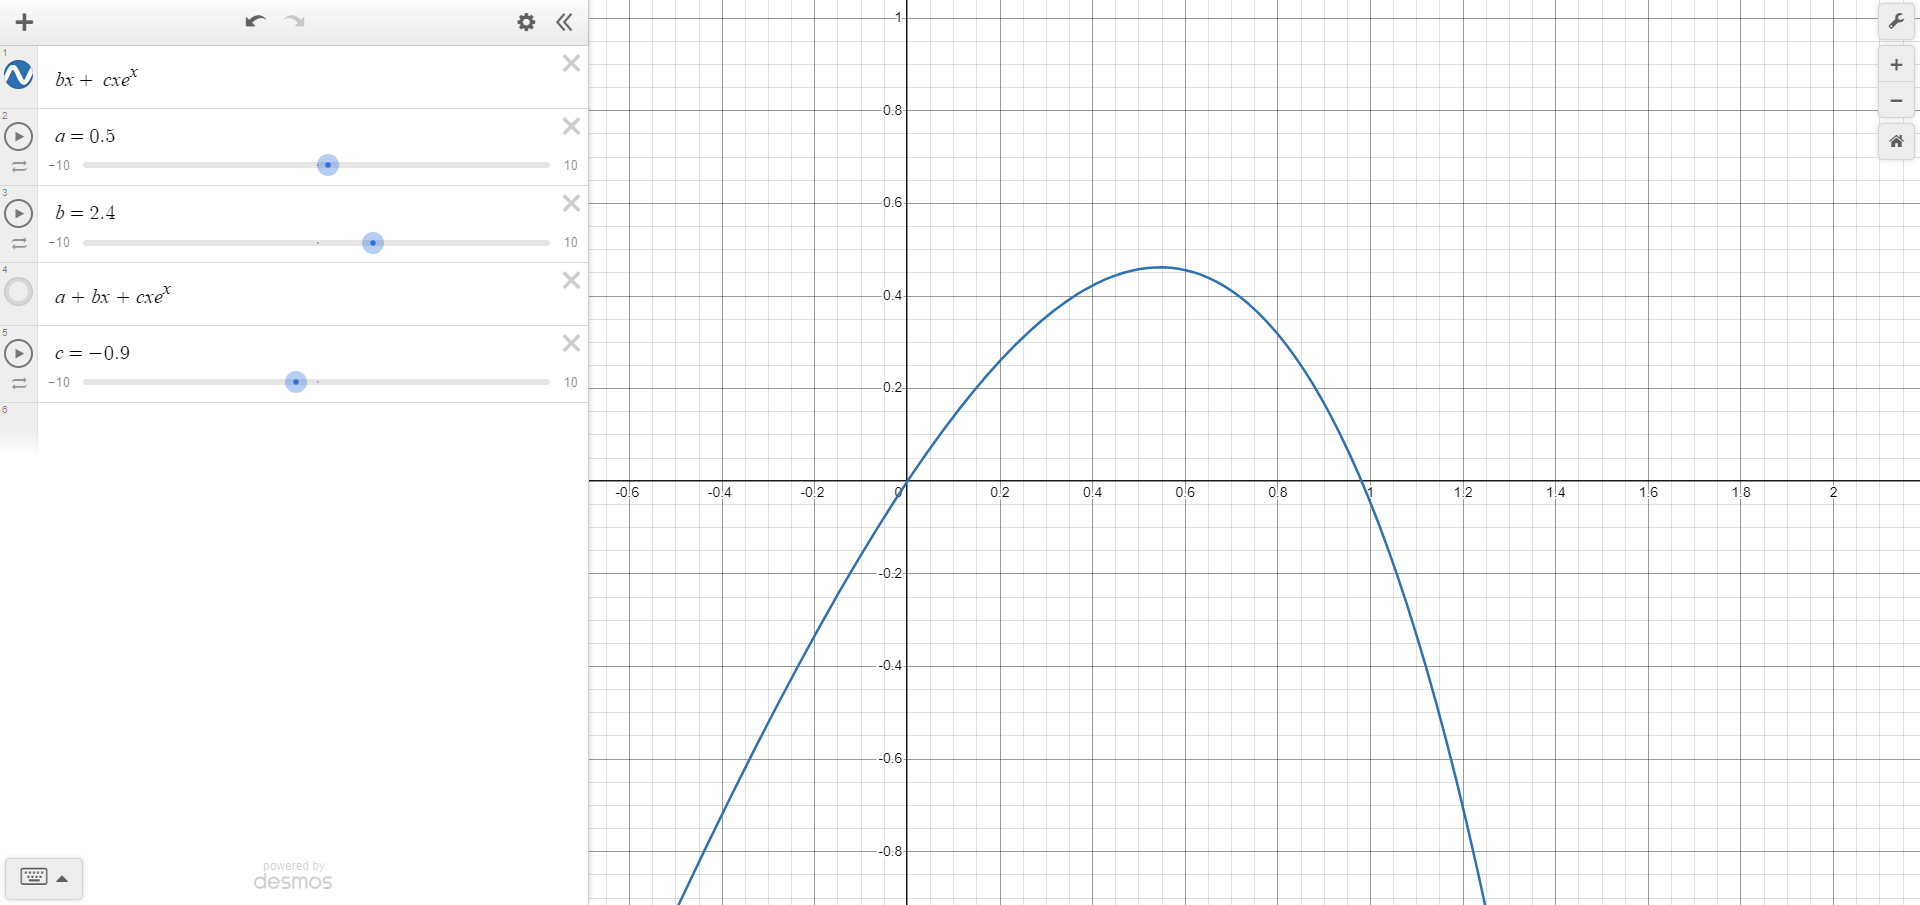
\includegraphics[width = 0.7\textwidth]{Figures/Counterexample8.png}
\end{figure}
\clearpage

\newpage
\section{Exercise 9}
Show that if $\Omega$ contains a subset homeomorphic to the letter `Y', then $C(\Omega)$ cannot contain a Haar subspace of dimension greater than one.
\partbreak
\begin{solution}

    This exercise is a direct application of the Marihuber-Curtis Theorem. The problem itself is agnostic to its proof, aside from the choice of continuous paths of two points, which I will denote as $x_1, x_2$. For ease of symmetry, and reasoning, I will instead relate the problem to `$\perp$' over `Y'. This choice is simply by aesthetic. Furthermore, all logic will be spoken with respect to the homeomorphic structure of the output space. Without loss of generality, we choose $x_1$ to begin on the left side of $\perp$, and $x_2$ to lie on the right side of $\perp$. These initial points are arbitrary, since the path chosen simply does not care about the distribution of $x_1, x_2$. With this in mind, we begin by considering the point which lies closest to the fork, and construct its path $\gamma_1$, to begin at $x_1$ and remain there for an arbitrarily long time, setting its derivative along the fork significantly less in magnitude than off the fork. At time $t\star_1$, we mark as the time that the curve $\gamma_1$ enters the fork, to which we begin the curve $\gamma_2$. The curve $\gamma_2$ will start, naturally, at $x_2$, and proceed laterally until it passes the fork. This time, which I will denote by $t\star_2$, should also mark the time where the derivative of $\gamma_1$ hits zero along the fork. The curve $\gamma_1$ will now mirror itself, until the points $\gamma_1$ and $\gamma_2$ pass. This ensures that the points $x_1$ and $x_2$ do not intersect along their respective trajectories. I have included an image below, done in paint, that conveys the paths described.
\end{solution}

\begin{figure}[!ht]
    \centering
    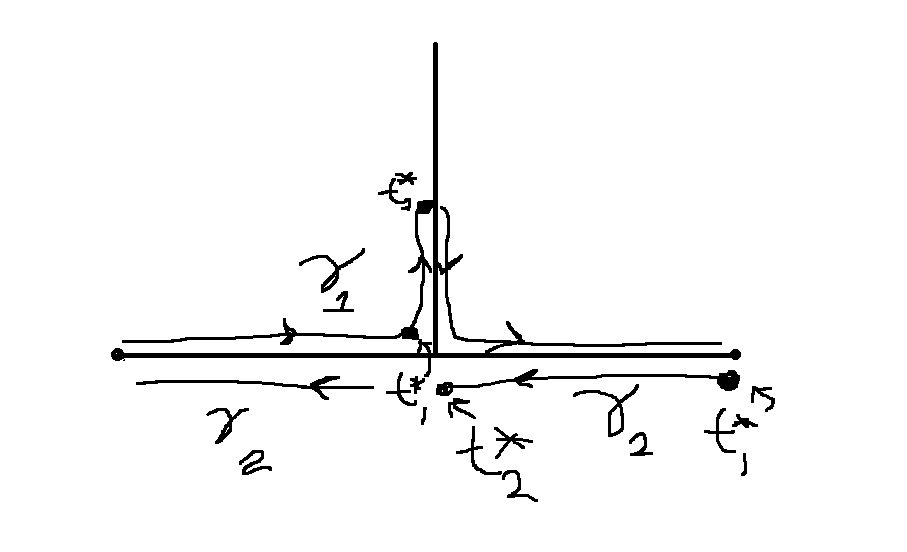
\includegraphics[width = 0.7\textwidth]{Figures/Exercise 9.png}
    \caption{Visual aid to describe the two proposed curves. The points $t_1\star$ and $t_2\star$ are labelled respectively on each curve $\gamma_1$ and $\gamma_2$.}
\end{figure}

\newpage
\section{Exercise 10}
Given $x_1, ..., x_n \in \R$, find an expression for the determinant of the $n\times n$ matrix $V$ with $(i, j)$-th entry $x_i^{j-1}$. Use this to show that the monomials form a Haar subspace.
\partbreak
\begin{solution}

    We first need to show the determinant is given as a simple form. I will explicitly work out an example below, where $n = 3$, and generalize it after to any $n$. We have then that 
    \[A =\mqty[1&x_1&x_1^2\\1&x_2&x_2^2\\1&x_3&x_3^2]\]
    Noting that the determinant of a matrix is invariant under linear combinations of rows and columns, we can cancel out the first column so that we have
    \[A = \mqty[0&x_1 - x_3&x_1^2 - x_3^2\\0&x_2 - x_3&x_2^2 - x_3^2\\1&x_3&x_3^2].\]
    The determinant will then be taken down the first column, so that we have
    \[\det A = (x_1 - x_3)(x_2^2 - x_3^2) - (x_2 - x_3)(x_1^2 - x_3^2).\]
    After some rearranging, ...
    \begin{align*}
        &(x_1 - x_3)(x_2^2 - x_3^2) - (x_2 - x_3)(x_1^2 - x_3^2)\\
        &(x_1 - x_3)(x_2 - x_3)(x_2 + x_3) - (x_2 - x_3)(x_1 - x_3)(x_1 + x_3)\\
        &(x_1 - x_3)(x_2 - x_3)(x_2 + x_3 - x_1 - x_3)\\
        &(x_3 - x_1)(x_2 - x_3)(x_1 - x_2)\\
        &(x_1 - x_2)(x_2 - x_3)(x_3 - x_1)
    \end{align*}
    we see that the determinant of $A$ is a product of permutations of the different points. Furthermore, due to the cyclic nature of the differences, each point $x_i$ appears twice in the polynomial. Therefore, the polynomial will be degree 6, when summing over all squares. Naturally, this procedure can be applied to any number of given points, except for the argument of the degree of the polynomial. Here, we should note that the highest single degree for $n = 3$ is 3, since when expanding the first line in the procedure above will give us $x_3^3$. Since we have $n$ points, the highest single degree we will encounter is $n$. Note that each column in the matrix will have degree $i$, thus, when summing over all columns, we get at total degree of $\frac{1}{2}(n)(n+1)$. Therefore, I propose the determinant for any given $n$ points to be 
    \[\det A = \prod_{1 \leq i < j \leq n} (x_j - x_i).\]

    This follows from the observation for $n = 3$. Once we have this, we are done. This is because the matrix $(\Phi)_{i, j} = u_j(x_i)$ formed by the basis of the monomials is the Vandermonde matrix, which is shown above to have nonzero determinant for distinct points $x_i, i \leq n$. Therefore, the monomials form a Haar subspace. 
\end{solution}


\newpage
\section{Exercise 11}
Let $\lm_1, ..., \lm_n \in \R_+$ and consider the set of functions $u_j: \R_+ \to \R_+$ with $u_j(x) = e^{-\lm_j x}$. Show that the $u_j$ are linearly independent and form a Haar subspace of $C(\R_+)$. 
\partbreak
\begin{solution}


    We will first show linear independence of the $u_j$'s. This will be done via induction on $n$. Denote $S_n$ to be the set containing the $u_i$ for $i \leq n$. 
    \begin{itemize}
        \item \underline{Base Case}: $n = 1$

        \hop
        The base case just boils down to assuming all $u_j$'s are nonzero. This is clear. Thus the base case is shown.

        \item \underline{Induction Hypothesis}

        \hop 
        Next, assume this holds for some $k$ collection of these functions, where $k<n$. That is, $S_k$ is a linearly independent set. We will next show that $S_{k+1}$ is a linearly independent set.

        \item \underline{Case}: $n = k+1$

        \hop
        Suppose false, that is, adding the $u_{k+1}$ basis vector makes the span of $S_{k+1}$ to be a linearly dependent set. This implies there exists $c_1, ..., c_k \neq 0$ for which
        \[\sum_{i = 1}^k c_iu_i(x) = u_{k+1},\]
        note the coefficient on the $u_{k+1}$ can be discarded. Suppose without loss of generality, $\lm_{k+1}$ is chosen to have the least value of all $\lm_i$'s. By substituting in the basis vectors, as well as multiplying each side by $e^{\lm_{k+1}x}$, we have
        \[\sum_{i = 1}^k c_ie^{(\lm_{k+1} - \lm_i)x} = 1 \quad \text{ for all } x \in \R_+.\]
        Since this should hold for all $x$, we can evaluate this function for two different values, namely $x = 0, 1$. This implies 
        \begin{align*}
            &\sum_{i = 1}^k c_i = 1\\
            &\sum_{i = 1}^k c_i e^{(\lm_{k+1} - \lm_i)} = 1
        \end{align*}
        Taking the second line, we investigate its absolute value. 
        \[1 = \abs{\sum_{i = 1}^k c_i e^{\lm_{k+1} - \lm_i}} \leq \max_i e^{\lm_{k+1} - \lm_i} \abs{\sum_{i = 1}^k c_i} = \max_i e^{\lm_{k+1} - \lm_i} \leq 1.\]
        The last inequality holds from us supposing that $\lm_{k+1}$ is bounded above by any other $\lm_i$. Since we get 1 on both sides, we can replace all inequalities with equalities, implying that 
        \[\max_i e^{\lm_{k+1} - \lm_i} = 1 \implies \text{argmax}_i (e^{\lm_{k+1} - \lm_i}) = 0.\]
        Therefore, $\lm_i = \lm_{k+1}$, for $i \leq k$. This is a contradiction, since we suppose that each $\lm_i$ is distinct. Therefore, span$(S_{k+1})$ is a linearly independent set. 
    \end{itemize}

    Next, we show that the $u_j$'s form a Haar subspace of $C(\R_+)$. That is, we need to show that any $u \in \text{span} (S_{k+1})$ has at most $n-1$ zeros in $\R_+$. Again, we will show this by induction. 
    \begin{itemize}
        \item \underline{Base case}: $n = 1$

        \hop
        Here, we suppose that $u \in S_n$ is just a multiple of only one $u_i$, thus $u = cu_i$ for some scalar $c$. To satisfy the definition of a Haar subspace, we demand that $u$ can have no zeros. Since $u_i(x) > 0$ for all $x \in \R_+$, we have that $cu_i(x)$ attains no zeros (assuming $c$ is nonzero). Therefore, the base case has been shown.  

        \item \underline{Induction Hypothesis}

        \hop 
        Next, assume this holds for some $k$ collection of $u_j$'s. That is, for $u \in \text{span}(S_k)$, $u$ has at most $k-1$ zeros. Suppose we take $u_{k+1}$ as an additional basis function, linearly independent from the other $u_j$'s (this can be done since we showed this property). Denote $S_{k+1} = \{u_j : 1 \leq j \leq k+1\}$. For $v \in \text{span}(S_{k+1})$, we will show that $v$ has at most $k$ zeros.

        \item \underline{Case}: $n = k+1$

        \hop
        Suppose false, that is, there exists a $v \in \text{span}(S_{k+1})$ which has $k+1$ zeros. That is, there exists $a_1, a_2, ..., a_{k+1} \in \R_+$ satisfying $v(a_1) = v(a_2) = ... = v(a_k) = v(a_{k+1}) = 0$. Pick $z_i \in (a_i, a_{i+1})$ for $i = 1, 2, ..., k$. By Rolle's Theorem, we can choose these $z_i$'s such that they satisfy
        \[v'(z_i) = 0, \quad i = 1, 2, ..., k\]
        Since $v \in \text{span}(S_{k+1})$, and $S_{k+1}$ has a linearly independent basis, we can choose $c_1, ..., c_{k+1} \in \R$ such that $v = \sum_{i = 1}^{k+1} c_i u_i$. Then, by differentiating, 
        \[\frac{d}{dx}v = \sum_{j = 1}^{k+1} c_j \frac{d}{dx}u_j = -\sum_{j = 1}^{k+1} c_j \lm_j u_j.\]
        Evaluating at the $z_i$'s, the following system can be written:
        \begin{align*}
            &-c_1\lm_1u_1(z_1) - c_2\lm_2u_2(z_1) - ... - c_{k+1}\lm_{k+1}u_{k+1}(z_1) = 0\\
            &-c_1\lm_1u_1(z_2) - c_2\lm_2u_2(z_2) - ... - c_{k+1}\lm_{k+1}u_{k+1}(z_2) = 0\\
            &\dots\\
            &-c_1\lm_1u_1(z_k) - c_2\lm_2u_2(z_k) - ... - c_{k+1}\lm_{k+1}u_{k+1}(z_k) = 0\\
        \end{align*}
        Note that, in the land of linear algebra, this system can be written in the form $Ax = b$, where $A$ is size $(k+1, k)$. This clearly implies $A$ is not invertible. Thus, there exists a column of $A$ which is linearly dependent on the previous columns, by the induction hypothesis, this column is the last column. Thus, for any $i$, we have that 
        \[-c_1\lm_1u_1(z_1) - c_2\lm_2u_2(z_1) - ... = c_{k+1}\lm_{k+1}u_{k+1}(z_1).\]
        Note that the $u_j$ are chosen as linearly independent. So the coefficients $c_i\lm_i$ are equal zero. This implies $c_i = 0$ or $\lm_i = 0$ both of which are contradictions. Thus, $v$ cannot possibly have $k+1$ zeros, so $v$ has at most $k$ zeros. This then proves the induction hypothesis. 
    \end{itemize}
\end{solution}

\newpage
\section{Exercise 12}
In this problem we will explore weighted spaces. In the following , assume $f$ is a continuous function on an interval $[a, b]$ and $w$ is a positive continuous weight function on $[a, b]$. For $p \in [1, \infty]$, let $\norm{\cdot}_p$ be defined by 
\[\norm{f}_p = \left(\int_a^b |f(x)|^p w(x) \ dx\right)^{1/p}.\]
For $p = 2$ we also define $\braket{\cdot}{\cdot}_w$ by 
\[\braket{f}{g} = \int_a^b f(x)g(x) w(x) \ dx.\]

\subsection{Exercise 12, part 1}
Show that for any $f \in C[a, b]$, $\norm{f}_1 \leq c\norm{f}_2$ and $\norm{f}_2 \leq c\norm{f}$, where 
\[c = \left(\int_a^b w(t) \ dt\right)^{1/2}.\]
Here, $\norm{\cdot}$ denotes the usual sup norm for $C([a, b])$. 
\partbreak
\begin{solution}

    I will first show the second inequality. This is shown via usual methods for the sup-norm. In particular, we note that 
    \[\int_a^b |f(x)|^2 w(x) \ dx \leq \int_a^b \left( \sup_{x \in [a, b]} |f(x)|\right)^2 w(x) \ dx = \left( \sup_{x \in [a, b]} |f(x)|\right)^2 \int_a^b w(x) \ dx\]
    The constant dragged out of the integral is exactly the squares sup norm of $f$. Performing the above line of equalities requires us to square the weighted two-norm of $f$ so that
    \[\norm{f}_{2, w}^2 = \int_a^b |f(x)|^2 w(x) \ dx .\]
    Therefore, noting that $c^2$ is just the integral of the weight function over the interval, we have that 
    \[\norm{f}_{2, w}^2 \leq c^2\norm{f}^2 \iff \norm{f}_{2, w} \leq c\norm{f}.\]
    For the first inequality, we relate the given 1-norm to the standard $L^1$ norm. Since the weight function is positive, its square root is defined over the real line. Next, observe
    \[\norm{f}_{1, w} = \int_a^b |f(x)| w(x) \ dx =  \int_a^b |f(x) w(x)| \ dx = \norm{fw}_{L^1}.\]
    By H\"older's inequality, setting $p = q = 2$, we have, 
    \[\norm{fw}_{L^1}^2 \leq \norm{f\sqrt{w}}_{L^2}^2 \norm{\sqrt{w}}_{L^2}^2,\]
    so when expanding, we see
    \[\norm{f\sqrt{w}}_{L^2}^2 \norm{\sqrt{w}}_{L^2}^2 = \left(\int_a^b |f(x)\sqrt{w(x)}|^2 \ dx \right)\left( \int_a^b |\sqrt{w(x)}|^2 \ dx\right).\]
    After simplification, 
    \[\norm{f\sqrt{w}}_{L^2}^2 \norm{\sqrt{w}}_{L^2}^2 = \left(\int_a^b |f(x)|^2 w(x) \ dx\right) \left(\int_a^b w(t) \ dt\right) = \norm{f}_{2, w} c^2 .\]
    Therefore, $\norm{f}_{1, w} \leq c \norm{f}_{2, w}$ after taking the square root on each side. Which is what we wanted to get. 
    
\end{solution}


\newpage
\subsection{Exercise 12, part 2}
Show that the polynomials are dense in $C([a, b])$ under all three norms $\norm{\cdot}$, $\norm{\cdot}_1$, and $\norm{\cdot}_2$. Show that $C([a, b])$ is not complete under $\norm{\cdot}_1$ or $\norm{\cdot}_2$. 
\partbreak
\begin{solution}

    I completed the first part before being told that this problem is optional. I will just turn in what I already have. 
\end{solution}
\newcommand{\pstar}{p_*}

\newpage
\section{Exercise 13}
For any $n \geq 0$ show that the mapping which takes the function $f\in C([-1, 1])$ to its best polynomial approximation $\pstar \in P_n$ is continuous with respect to the $\infty$-norm on $C([-1, 1])$.
\partbreak
\begin{solution}

    The proof that I am about to give might be completely wrong. It utilizes the Stone weierstrass theorem, which states that any function on $C([-1, 1])$\footnote{The notes mention the theorem to hold on $C([0, 1])$, which has been mentioned in class the chosen interval is arbitrary.} has a polynomial $p$ such that their distance can be made less than epsilon. \par

    \jump
    Suppose that we have a sequence of functions in $C([-1, 1]), f_n$ which converge to $f$. We are guaranteed this sequence exists since the space $C([-1, 1])$ is a Banach space, hence complete. We wish to find a $\delta$ for which, when $n \geq N$, $\norm{P(f_j) - P(f)} < \ep$. Let $\delta = \ep / 3$; by adding two zeros to the latter norm, we have
    \begin{align*}
        \norm{P(f_j) - P(f)} &= \norm{P(f_j) - P(f) + f_j - f - f_j + f}\\
        &\leq \norm{P(f_j) - f_j} + \norm{f - P(f)} + \norm{f_j - f} \\
        &< \frac{1}{3}(\ep + \ep + \ep)\\
        &= \ep
    \end{align*}
    
    Note that the first and second norms are bounded by $\ep$ by the Stone Weierstrass theorem, where $\ep$ is chosen to be the supremum over all $\ep$ of the sequence $f_j$. Therefore, the mapping is continuous.  
\end{solution}
\newcommand{\xstar}{x_*}



\newpage
\section{Exercise 15}
A (simplified) Remez algorithm works by doing the following: Choose "control" points $x_0, ..., x_{n+1}$ in the interval $[0, 1]$ to initialize. For each iteration, form the system
\[
\mqty[1 &x_0&x_0^2&\dots &x_0^n&-1\\
      1 &x_1&x_1^2&\dots &x_1^n& 1\\
      \vdots&\vdots&\ddots  &     &  \\
      1&x_{n+1}&x_{n+1}^2&\dots&x_{n+1}^n&(-1)^{n+2}] 
\mqty[\alpha_0\\\vdots\\\alpha_n\\E] = \mqty[f(x_0)\\ \vdots\\f(x_{n+1})]
\]
and solve it. Find the location of the maximum $e(x) = f(x) - \sum_{j = 0}^n\alpha_j x^j$ on the interval $[0, 1]$. Call it $\xstar$. Move the closest control point $x_i$ (for which the signs of $e(\xstar)$ and $e(x_i)$ agree) to $\xstar$ and move to the next iteration.  
\subsection{Exercise 15, part 1}
Perform one iteration of the Remez algorithm to compute the best polynomial approximation to $x^5$ on by polynomials of degree at most 3 on the interval $[0, 1]$. Start with equispaced nodes $x_0 = 0, ..., x_4 = 1$. 
\partbreak
\begin{solution}

    For equally spaced nodes over the interval $[0, 1]$, we initialize with the distribution $x_i = i/4$. For this distribution, we have the given matrix, which I will denote as $A$, is expressed by 
    \[A = \mqty[
      1 &x_0&x_0^2&x_0^3&-1\\
      1 &x_1&x_1^2&x_1^3& 1\\
      1 &x_2&x_2^2&x_2^3& -1\\
      1 &x_3&x_3^2&x_3^3& 1\\
      1 &x_4&x_4^2&x_4^3& -1] = 
      \mqty[
      1 &0&0&0&-1\\
      1 &(0.25)&(0.25)^2&(0.25)^3&1\\
      1 &(0.5)&(0.5)^2&(0.5)^3& -1\\
      1 &(0.75)&(0.75)^2&(0.75)^3& 1\\
      1 &1&1&1& -1]  
      \]
      Therefore, with the given function evaluation at each $x_i$, we have the following system:
      \[
      \mqty[
      1 &0&0&0&-1\\
      1 &(0.25)&(0.25)^2&(0.25)^3&1\\
      1 &(0.5)&(0.5)^2&(0.5)^3& -1\\
      1 &(0.75)&(0.75)^2&(0.75)^3& 1\\
      1 &1&1&1& -1]  
      \mqty[
      \alpha_0\\
      \alpha_1\\
      \alpha_2\\
      \alpha_3\\
      E] = 
      \mqty[
      0\\
      (0.25)^5\\
      (0.5)^5\\
      (0.75)^5\\
      1].
      \]
      Solving this system (using Wolfram Alpha), we get the following solution to the system:
      \[\mqty[\alpha_0\\\alpha_1\\\alpha_2\\\alpha_3\\E] = \mqty[-0.0146484\\0.53125\\-2.34375\\2.8125\\-0.0146484]\]
      For the Remez Algorithm, the first iteration of coefficients over a uniform distribution of points over the given interval is shown in Figure \ref{fig:firstRemez15}. This does a decent job of approximating the function, however we see the local maxima in the error function are not at equal height. The points for which the local minima appear are roughly around $x = 0.155, 0.512, 0.860$. Since the local maxima do not achieve the same height, further iterations of the Remez algorithm is required; we then find the point from our original spread which is closest to any of these local maxima and replace it. Upon inspection, we see that the point marked $x_1 = 0.25$ should be replaced with the local maxima $0.155$. We then repeat the algorithm until all local maxima achieve the same height \textit{and} they oscillate. 
\end{solution}
\vspace{1in}
\begin{figure}[!hb]
    \centering
    \begin{subfigure}
    \centering
        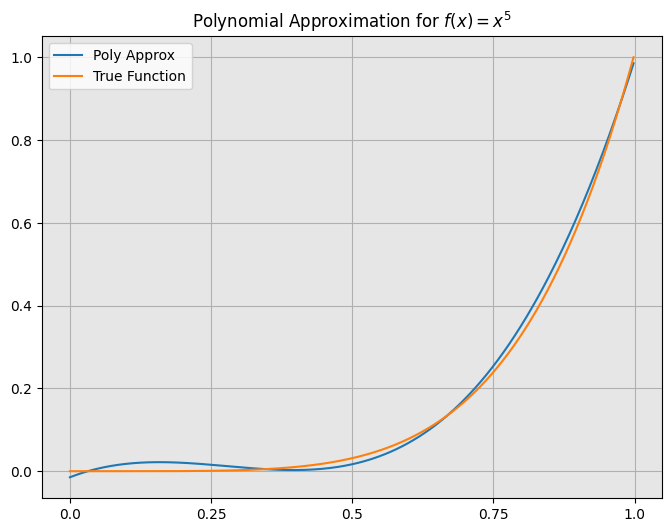
\includegraphics[width=0.35\textwidth]{Figures/FirstRemez15.png}     
    \end{subfigure}%
    \hspace{10mm}
    \begin{subfigure}
        \centering
        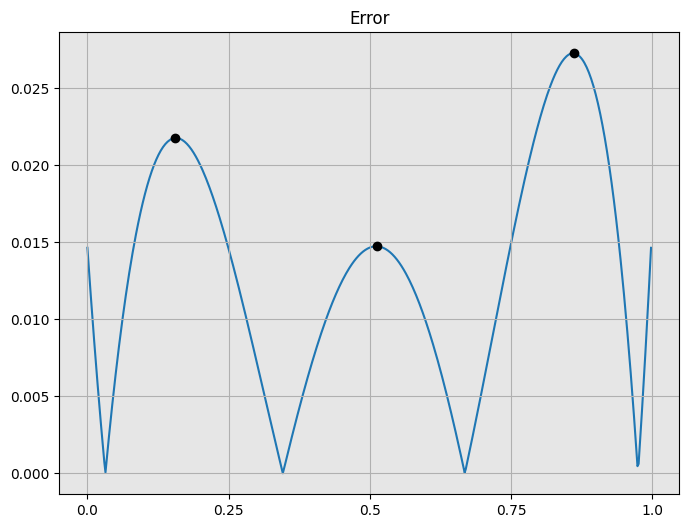
\includegraphics[width=0.35\textwidth]{Figures/Error15.png}    
    \end{subfigure}
    \caption{The first iteration of the Remez Algorithm for $f(x) = x^5$. The coefficients and error are given above. Figure 2: Error for the first iteration. Local maxima are given in black.}
    \label{fig:firstRemez15}
\end{figure}



\newpage
\subsection{Exercise 15, part 2}
Write a code to use the Remez algorithm to compute the best polynomial approximation to $x^5$ by polynomials of degree at most 3 on the interval [0, 1]. Plot the equioscillation points and the error as a function of iteration number. Show plots for initialization both with equispaced points and random initial points.
\partbreak
\begin{solution}

    I have (hopefully) implemented the Remez algorithm correctly, using either a uniform distribution of initial points or a random distribution (uniform distribution, apologies for the overlap in terminology). The uniform distribution is shown in Figure \ref{fig:RemezFinal}, next to the random distribution of points. The random initization did not produce an egregiously bad polynomial, which can happen for initial points being too close to each other.  
\end{solution}

\vspace{1in}
\begin{figure}[!hb]
\centering
    \begin{subfigure}
        \centering
        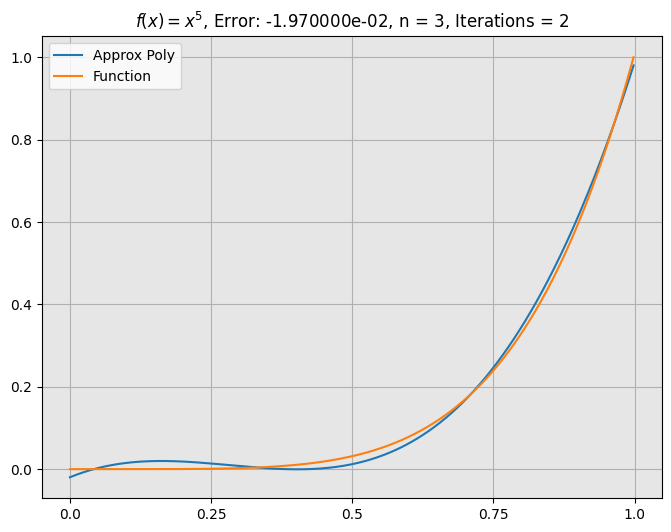
\includegraphics[width = 0.4\textwidth]{Figures/RemezFinalUnif.png}
    \end{subfigure}
    \begin{subfigure}
        \centering
        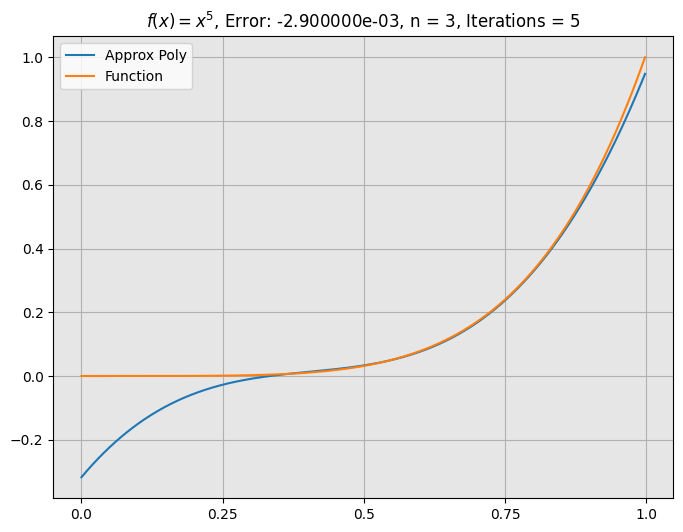
\includegraphics[width = 0.4\textwidth]{Figures/RemezFinalRandom.png}
    \end{subfigure}
    \caption{The Remez algorithm initialized with (left) uniform points and (right) random points. Iterations, degree, and Error are given in each}
    \label{fig:RemezFinal}
\end{figure}

\newpage
\subsection{Exercise 15, part 3}
Extend your code in some way (multiple points at once, more general function, more stable formulae for solving the linear system, some different experiments, etc.).
\partbreak
\begin{solution}

    I have written my code flexible enough to work on any given function (within reason). I have also taken into consideration numerical stability with respect to solving the system of equations. I am solving the system via LU decomposition with partial pivoting, then solving. I have tested my algorithm on the Heavyside function, using a polynomial of degree 30, and investigating the first, second, and 4000-th iteration of the algorithm. The output is given below. Note that I cut off the edges of the domain so we can see the influence of each iteration. 
\end{solution}
\vspace{1in}
\begin{figure}[!hb]
    \centering
    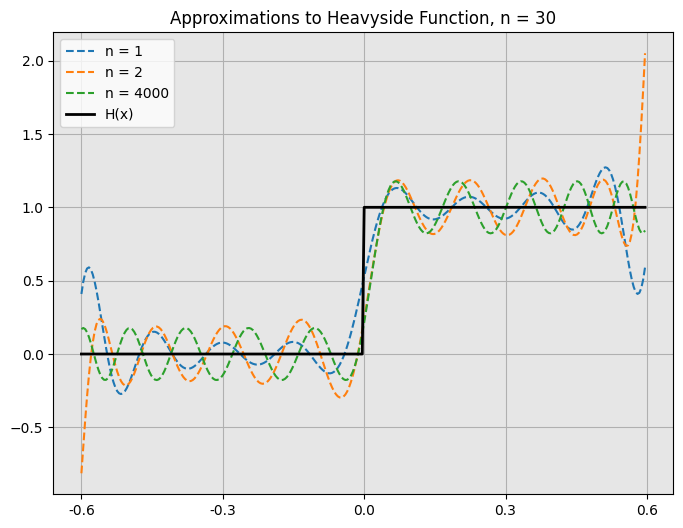
\includegraphics[width = 0.6\textwidth]{Figures/RemezHeavyside.png}
    \caption{Approximations to Heavyside function. The error on the 4000-th iterate is roughly -0.17. The behavior of the error changes drastically for different degree approximations.}
    \label{fig:RemezHeavyside}
\end{figure}
\clearpage



\newpage
\section{Exercise 16}
Recall the formula for Chebyshev polynomials:
\[T_n(x) = \cos(n\arccos(x)).\]
\subsection{Exercise 16, part 1}
Let $p \in P_n$ be a polynomial given by a finite Chebyshev series
\[p(x) = \sum_{k = 0}^n \alpha_k T_k(x)\]
and let $s \in [-1, 1]$. Show that $p(s)$ can be evaluated using the following algorithm. Set $u_{n+1} = 0, u_n = \alpha_n$ and 
\[u_k = 2su_{k+1} - u_{k+2} + \alpha_k, \quad k = n - 1, n - 2, ..., 0.\]
Then $p(s) = \frac{1}{2}(\alpha_0 + u_0 - u_2).$
\partbreak
\begin{solution}

    We will go straight into calculations. 
    \tightalignbreak
\begin{align*}
    &u_0 - u_2 + \alpha_0 = 2su_1 - 2u_2 + 2\alpha_0 &\text{(First recurrence.)}\\
    &= 2s(2su_2 - u_3 + \alpha_1) - 2u_2 + 2\alpha_0 &\text{(Second recurrence.)}\\
    &= 2(2s^2 - 1)u_2 - 2su_3 + 2s\alpha_1 + 2\alpha_0 &\text{(Simplifying.)}\\
    &\hspace{10mm}\rightarrow 2T_2(s)u_2 - 2T_1(s)u_3 + 2T_1(s)\alpha_1 + 2T_0(s)\alpha_0 &\text{(Rewriting, quick note.)}\\
    &= 2(2s^2 - 1)(2su_3 - u_4 + \alpha_2) - 2su_3 + 2s\alpha_1 + 2\alpha_0&\text{(Fourth recurrence.)}\\
    &= 2[(4s^3 - 3s)u_3] - 2[(2s^2 - 1)u_4] + 2(2s^2 - 1)\alpha_2 + 2s\alpha_1 + 2\alpha_0 &\text{(Simplifying.)}\\
    &\hspace{10mm}\rightarrow 2T_3(s)u_3(s) - 2T_2(s)u_4 + 2\left(\sum_{k = 0}^2 T_k\alpha_k\right) &\text{(Rewriting.)}\\
    &\hspace{1.5in}\vdots &\text{(Assuming holds.)}\\
    &= 2T_{n-1}(s)u_{n-1} - 2T_{n-2}u_n + 2\left(\sum_{k = 1}^{n-2}T_k(s)\alpha_k\right) &\text{((n-1)-th recursion.)}\\
    &= 2T_{n-1}(s)(2su_n - u_{n+1} + \alpha_{n-1}) - 2T_{n-2}u_n + 2\left(\sum_{k = 1}^{n-2}T_k(s)\alpha_k\right) &\text{(n-th recursion.)}\\
    &= 2\left[ (2sT_{n-1}(s) - T_{n-2})u_n + T_{n-1}\alpha_{n-1} + \sum_{k = 1}^{n-2}T_k(s)\alpha_k\right] &\text{(Simplifying.)}\\
    &= 2\left[T_n(s)u_n + T_{n-1}\alpha_{n-1} + \sum_{k = 1}^{n-2}T_k(s)\alpha_k\right] &\text{(Recurrence for $T_n$.)}\\
    &= 2\left(\sum_{k = 0}^n T_k(s)\alpha_k\right)&\text{(Simplifying.)}\\
    &=2p(s) &\text{(Given.)}
\end{align*}
\vspace{-12mm}\alignbreak
Therefore, $p(s) = \frac{1}{2}(u_0 - u_2 + \alpha_0)$. 

\end{solution}


\newpage
\subsection{Exercise 16, part 2}
Show that $T_n$ satisfies the ODE $(1 - x^2)y'' - xy' + n^2y = 0$.
\partbreak
\begin{solution}

    Taking the first two derivatives of $T_n$, we see
    \begin{align*}
        &\frac{dT_n}{dx} = \frac{d}{dx}\left(\cos(n\arccos(x))\right) = -sin(n\arccos(x))\frac{d}{dx}\left(n\arccos(x)\right) = \frac{n\sin(n\arccos(x))}{\sqrt{1 - x^2}}\\
        &\frac{d^2T_n}{dx^2} = -\sin(n\arccos(x))\left(n\frac{d}{dx^2}\left(\arccos(x)\right)\right) - n^2\left(\frac{d}{dx}\arccos(x)\right)^2\cos(n\arccos(x))\\
        &\hspace{10mm} = \frac{nx\sin(n\arccos(x))}{(1 - x^2)^{3/2}} - \frac{n^2T_n}{1 - x^2}
    \end{align*}
    When multiplying the second derivative by $(1 - x^2)$, the denominator on the second term cancels, and the first term's denominator is then a square root, we then get
    \[(1 - x^2)\frac{d^2T_n}{dx^2} = \frac{nx\sin(n\arccos(x))}{\sqrt{1 - x^2}} - n^2T_n.\]
    We can clearly see the first term is the first derivative multiplied by $x$. 
    \[(1 - x^2)\frac{d^2T_n}{dx^2} = x\frac{dT_n}{dx} - n^2T_n.\]
    By rearranging, we get that
    \[(1 - x^2)\frac{d^2T_n}{dx^2} - x\frac{dT_n}{dx} + n^2T_n = 0,\]
    which is what we wanted.
\end{solution}

\end{document}